\documentclass[tikz]{standalone}
\usepackage{tikz}
\usetikzlibrary{calc}
\usetikzlibrary{positioning}
\usetikzlibrary{fit}
\usetikzlibrary{backgrounds}

\definecolor{lightGreen}{HTML}{d5e8d4}
\definecolor{lightYellow}{HTML}{fff2cc}
\definecolor{lightGray}{HTML}{f5f5f5}
\definecolor{lightRed}{HTML}{ff9999}
\definecolor{lightBlue}{HTML}{d5e5fc}
\definecolor{lightCyan}{HTML}{a7dfe3}
\pgfdeclarelayer{main_bg}
\pgfdeclarelayer{back_bg}
\pgfsetlayers{back_bg,main_bg,main}

\newcommand{\metarect}[7]{
    \begin{scope}
        \node (#1) [rectangle, draw, text width=\rectWidth, minimum width=\rectWidth, minimum height=\rectHeight, #7] {};
        \node (#1_upper) [rectangle, draw, fill=#6, text width=\rectWidth, minimum width=\rectWidth, minimum height=\rectHeight*0.5, below=0.0pt of #1.north, anchor=north] {#2};
        \node (#1_middle) [rectangle, draw, fill=white, font=\tiny, text width=\rectWidth, minimum width=\rectWidth, minimum height=\rectHeight*0.25, below=-\the\pgflinewidth of #1_upper] {#3};
        \node (#1_bleft) [rectangle, draw, fill=white, font=\tiny, text width=\rectWidth*0.35, minimum width=\rectWidth*0.35, minimum height=\rectHeight*0.25, below=-\the\pgflinewidth of #1_middle.south west, anchor=north west] {#4};
        \node (#1_bright) [rectangle, draw, fill=white, font=\tiny, text width=\rectWidth*0.65, minimum width=\rectWidth*0.65, minimum height=\rectHeight*0.25, right=-\the\pgflinewidth of #1_bleft] {#5};
    \end{scope}
}

\begin{document}
    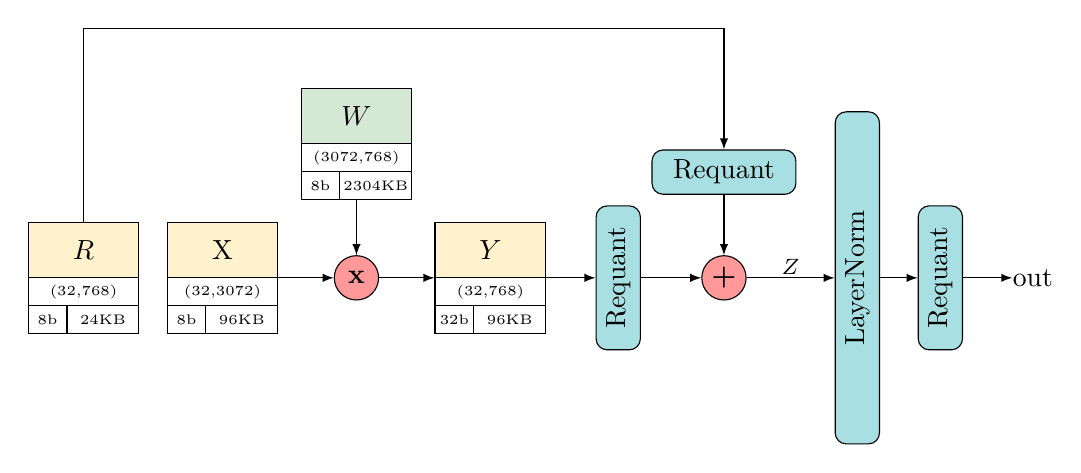
\begin{tikzpicture}[inner sep=0.0 pt, align=center]
    \pgfmathsetmacro{\rectWidth}{40}
    \pgfmathsetmacro{\rectHeight}{40}
    \pgfmathsetmacro{\multSize}{16 pt}

    \metarect{R}{$R$}{(32,768)}{8b}{24KB}{lightYellow}{}
    \metarect{X}{X}{(32,3072)}{8b}{96KB}{lightYellow}{right=\rectWidth*0.75pt of R.center}
    % \metarect{X}{X}{(32,3072)}{8b}{96KB}{lightYellow}{}
    \node [draw, circle, fill=lightRed, minimum size=\multSize, right=\rectWidth*0.5pt of X] (mult) {\textbf{x}};
    \metarect{Y}{$Y$}{(32,768)}{32b}{96KB}{lightYellow}{right=\rectWidth*0.5pt of mult}
    \node [draw, fill=lightCyan, rounded corners, minimum width=\rectHeight*1.3, minimum height=\rectWidth*0.4, rotate=90, right=\rectWidth*0.65pt of Y, anchor=center] (Y_req) {Requant};
    \node [draw, circle, fill=lightRed, minimum size=\multSize, right=\rectWidth*0.75pt of Y_req.center] (add) {\textbf{+}};
    \metarect{weight}{$W$}{(3072,768)}{8b}{2304KB}{lightGreen}{above=\rectHeight*0.5pt of mult}
    \node [draw, fill=lightCyan, rounded corners, minimum width=\rectHeight*1.3, minimum height=\rectWidth*0.4, above=\rectWidth*0.75pt of add, anchor=center] (R_req) {Requant};
    % \metarect{Z}{$Z$}{(32,768)}{32b}{96KB}{lightYellow}{right=\rectWidth*0.5pt of add}

    \draw [-latex] (X.east) -- (mult.west);
    \draw [-latex] (weight.south) -- (mult.north);
    \draw [-latex] (mult.east) -- (Y.west);
    \draw [-latex] (Y.east) -- (Y_req.north);
    \draw [-latex] (Y_req.south) -- (add.west);
    % \draw [-latex] (add.east) -- (Z.west);

    % \node (R) [above=\rectWidth*0.75pt of R_req] {$R$};
    % \draw [-latex] (R.south) -- (R_req.north);
    \draw [-latex] (R.north) -- ++(0pt,\rectHeight*1.75pt) -| (R_req.north);
    \draw [-latex] (R_req.south) -- (add.north);

    \node [draw, fill=lightCyan, rounded corners, minimum width=\rectHeight*3, minimum height=\rectWidth*0.4, rotate=90, right=\rectWidth*1pt of add, anchor=center] (ln2) {LayerNorm};
    \node [draw, fill=lightCyan, rounded corners, minimum width=\rectHeight*1.3, minimum height=\rectWidth*0.4, rotate=90, right=\rectWidth*0.75pt of ln2.center, anchor=center] (out_req) {Requant};
    % \metarect{out}{out}{(32,768)}{8b}{24KB}{lightYellow}{right=\rectWidth*0.65pt of out_req.center}
    \node (out) [right=\rectWidth*0.65pt of out_req.center] {out};

    \draw [-latex] (add.east) -- (ln2.north) node[midway, above, yshift=1pt, font=\footnotesize] {$Z$};
    % \draw [-latex] (Z.east) -- (ln2.north);
    \draw [-latex] (ln2.south) -- (out_req.north);
    \draw [-latex] (out_req.south) -- (out.west);
    % \draw [-latex] (out.east) -- ++(1,0);

%    \begin{pgfonlayer}{main_bg}
%        % fill=red!3
%        \node (all) [draw, rectangle, inner sep=40pt, fit=(layer_input)(weight_Q)(weight_K)(weight_V)(mixQ32b)(mixV32b)(Ci8b)(out)] {};
%    \end{pgfonlayer}
    \end{tikzpicture}

\end{document}
